\subsection{The $M_{1+}$ dominance assumption}
The approximation made  of $\ell$ up to d-waves
is a good approximation: one can see from \F{fig:Coefficients_q2.4}
that $A_4$, $C_1$, $D_2$ are rather small around the $\Delta$ compared to their
respectives coefficients with smaller $\ell$.
In order to make a model independent extraction of the multipoles a further approximation is needed.


Previous measurements at lower $Q^2$ showed that $E_{1+}$ and $S_{1+}$ are relatively small compared
to $M_{1+}$. All models that apply in this range of $Q^2$ show 
that $M_{1+}$ is the multipole that has the greatest strength.

The $M_{1+}$ dominance approximation consists in considering only  the multipoles
that interfere with $M_{1+}$.
With this approximation the relation between the Legendre coefficients and the electromagnetic multipoles
is \cite{bib:raskin}:
\begin{equation}
\begin{array}{l c l}
| M_{1+} |^2 & = & A_0/2 \\
Re(E_{1+}M_{1+}^*) & = & (A_2 - 2C_0/3)/8 \\
Re(S_{1+}M_{1+}^*) & = & D_1/6 \\
Re(E_{0+}M_{1+}^*) & = & A_1/2 \\
Re(S_{0+}M_{1+}^*) & = & D_0 \\
Re(M_{1-}M_{1+}^*) & = & -(A_2+2(A_0+C_0))/8 \\
\end{array}
\label{eqno:m1dominance}
\end{equation}

To obtain the various multipole ratios $\Re_{m}$ at the resonance peak, a Taylor expansion 
distribution around $M_W = 1.232$ $GeV$ is performed, as shown in \F{fig:multiem_taylor} \F{fig:multism_taylor}:
$$
\Re_{m} (W) \sim a_0 + a_1(x-M_W) + a_2(x-M_W)^2 + ...  = \sum_{i}a_i(x-M_W)^i
$$
with this expansion, at the $\Delta $ peak we have $\Re_{m} = a_0$.

\begin{figure}[h]
 \begin{center}
 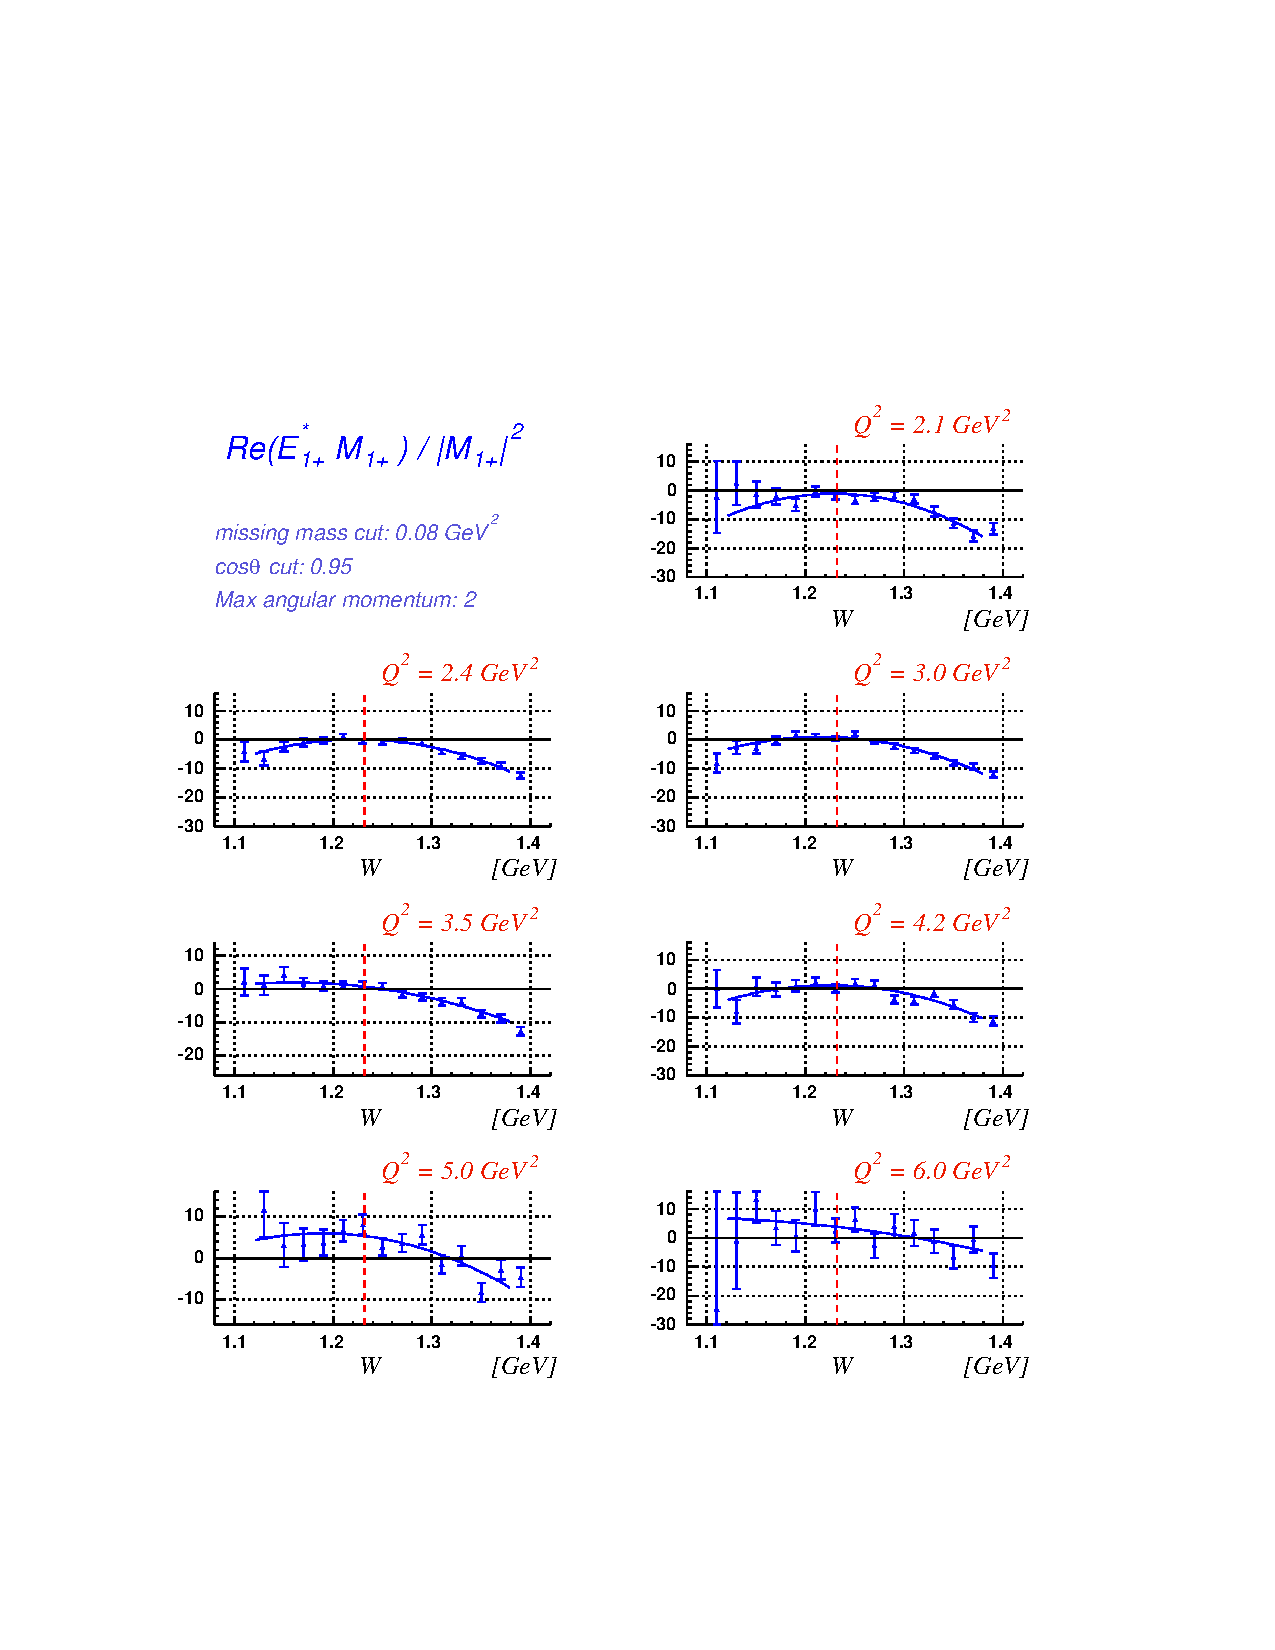
\includegraphics[width = 13cm, bb=30 130 550 600]{analysis/img/multiem_taylor} 
  \caption[ $Re(E_{1+}M_{1+}^*)$ as a function of $W$ for different $Q^2$.]
{ $Re(E_{1+}M_{1+}^*)$ as a function of $W$ for different $Q^2$. The value at the $\Delta $ peak
is the $a_0$ coefficient of the Taylor expansion around $M_W = 1.232$}
 \label{fig:multiem_taylor}
 \end{center}
\end{figure}
\begin{figure}[h]
 \begin{center}
 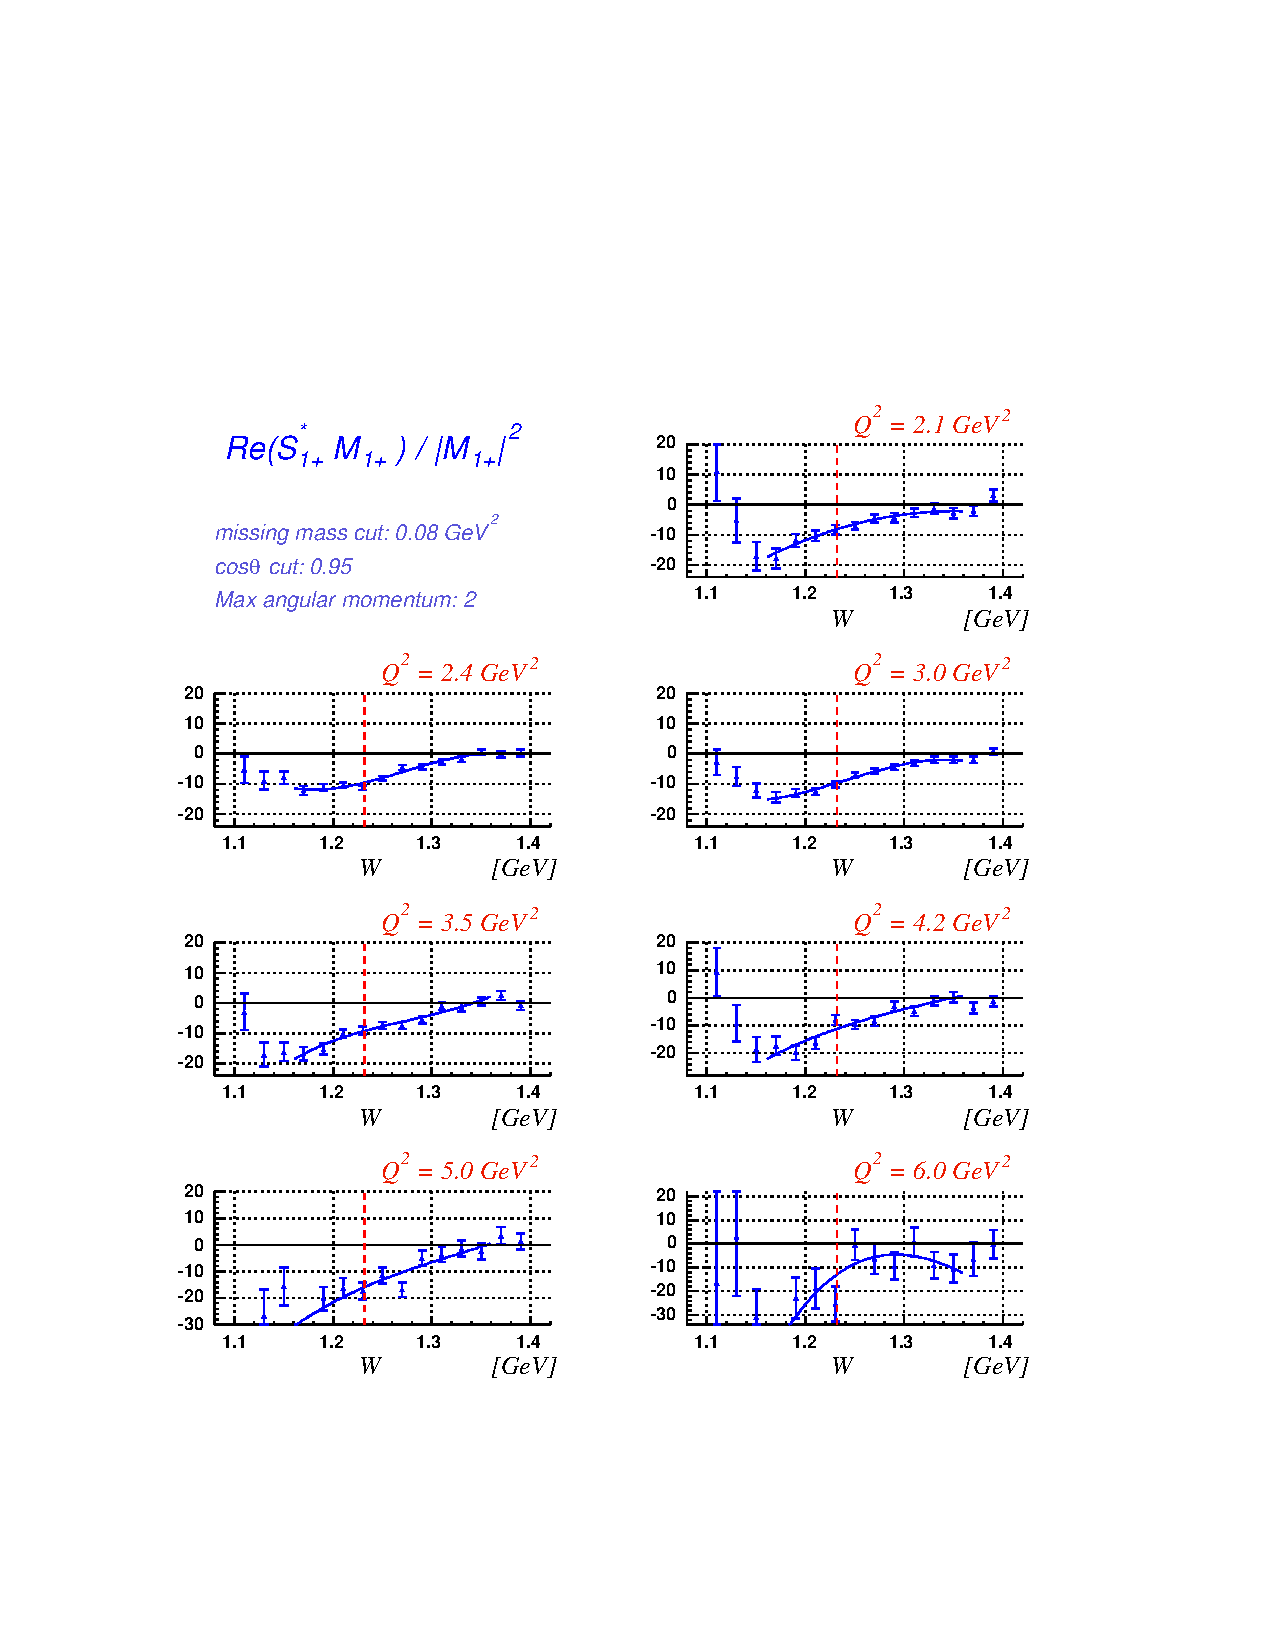
\includegraphics[width = 13cm, bb=30 130 550 600]{analysis/img/multism_taylor} 
  \caption[ $Re(S_{1+}M_{1+}^*)$ as a function of $W$ for different $Q^2$.]
{ $Re(S_{1+}M_{1+}^*)$ as a function of $W$ for different $Q^2$. The value at the $\Delta $ peak
is the $a_0$ coefficient of the Taylor expansion around $M_W = 1.232$}
 \label{fig:multism_taylor}
 \end{center}
\end{figure}
To see all the multipoles and multipoles ratios plots see
\begin{verbatim} 
http://www.jlab.org/~ungaro/pi0eprod/multipoles
\end{verbatim}



\subsection{ Effect of $M_{1+}$ dominance and $\ell \le 2$ approximation}
\label{sec:m1pdomeffect}
The $M_{1+}$ dominance assumption and
the limited order ($\ell \le 2$) in the Legendre expansion of the structure functions
introduce an uncertainty in the extraction of the multipoles which is expected to 
become greater with increasing $Q^2$.

In order to evaluate such uncertainty
two models (MAID, DMT) were used to generate the cross sections $\sigma_{MAID}$ and $\sigma_{DMT}$.
These models provide the multipoles $E_{\ell\pm}$, $S_{\ell\pm}$, $M_{\ell\pm}$ with $\ell$ up tp $5$.

The generated cross section were fitted as described in Section \ref{sec:structure} to extract
the structure functions. The structure functions were fitted
with orthogonal Legendre polynomials with $\ell$ up to d-waves as in Section \ref{sec:legendre}.
The approximation (\ref{eqno:m1dominance}) was used in order to extract the multipoles.

\F{fig:maid_comp} and \F{fig:dmt_comp} show the model and extracted multipole ratios for 
$Q^2$ = $3.5$ GeV$^2$.

One can see that in the $\Delta$ region DMT prescribes a smaller 
value of $S_{1+}$ then MAID.  The differences become even larger at higher $Q^2$.
$E_{1+}$ remains negative and constant for MAID while it becomes positive in DMT between $Q^2$ of $3$ and $4$
GeV$^2$.
\begin{figure}[h]
 \begin{center}
 \includegraphics[width = 15cm, bb=30 130 500 600]{analysis/img/multipoles_q2_3.5_data1}
  \caption[Comparison between the model (dashed blue line) and extracted (red points) multipole ratios for MAID 2000]
          { Comparison between the model and extracted multipole ratios for MAID 2000 at $Q^2$ = $3.5$ GeV$^2$.}
 \label{fig:maid_comp}
 \end{center}
\end{figure}

\begin{figure}[h]
 \begin{center}
 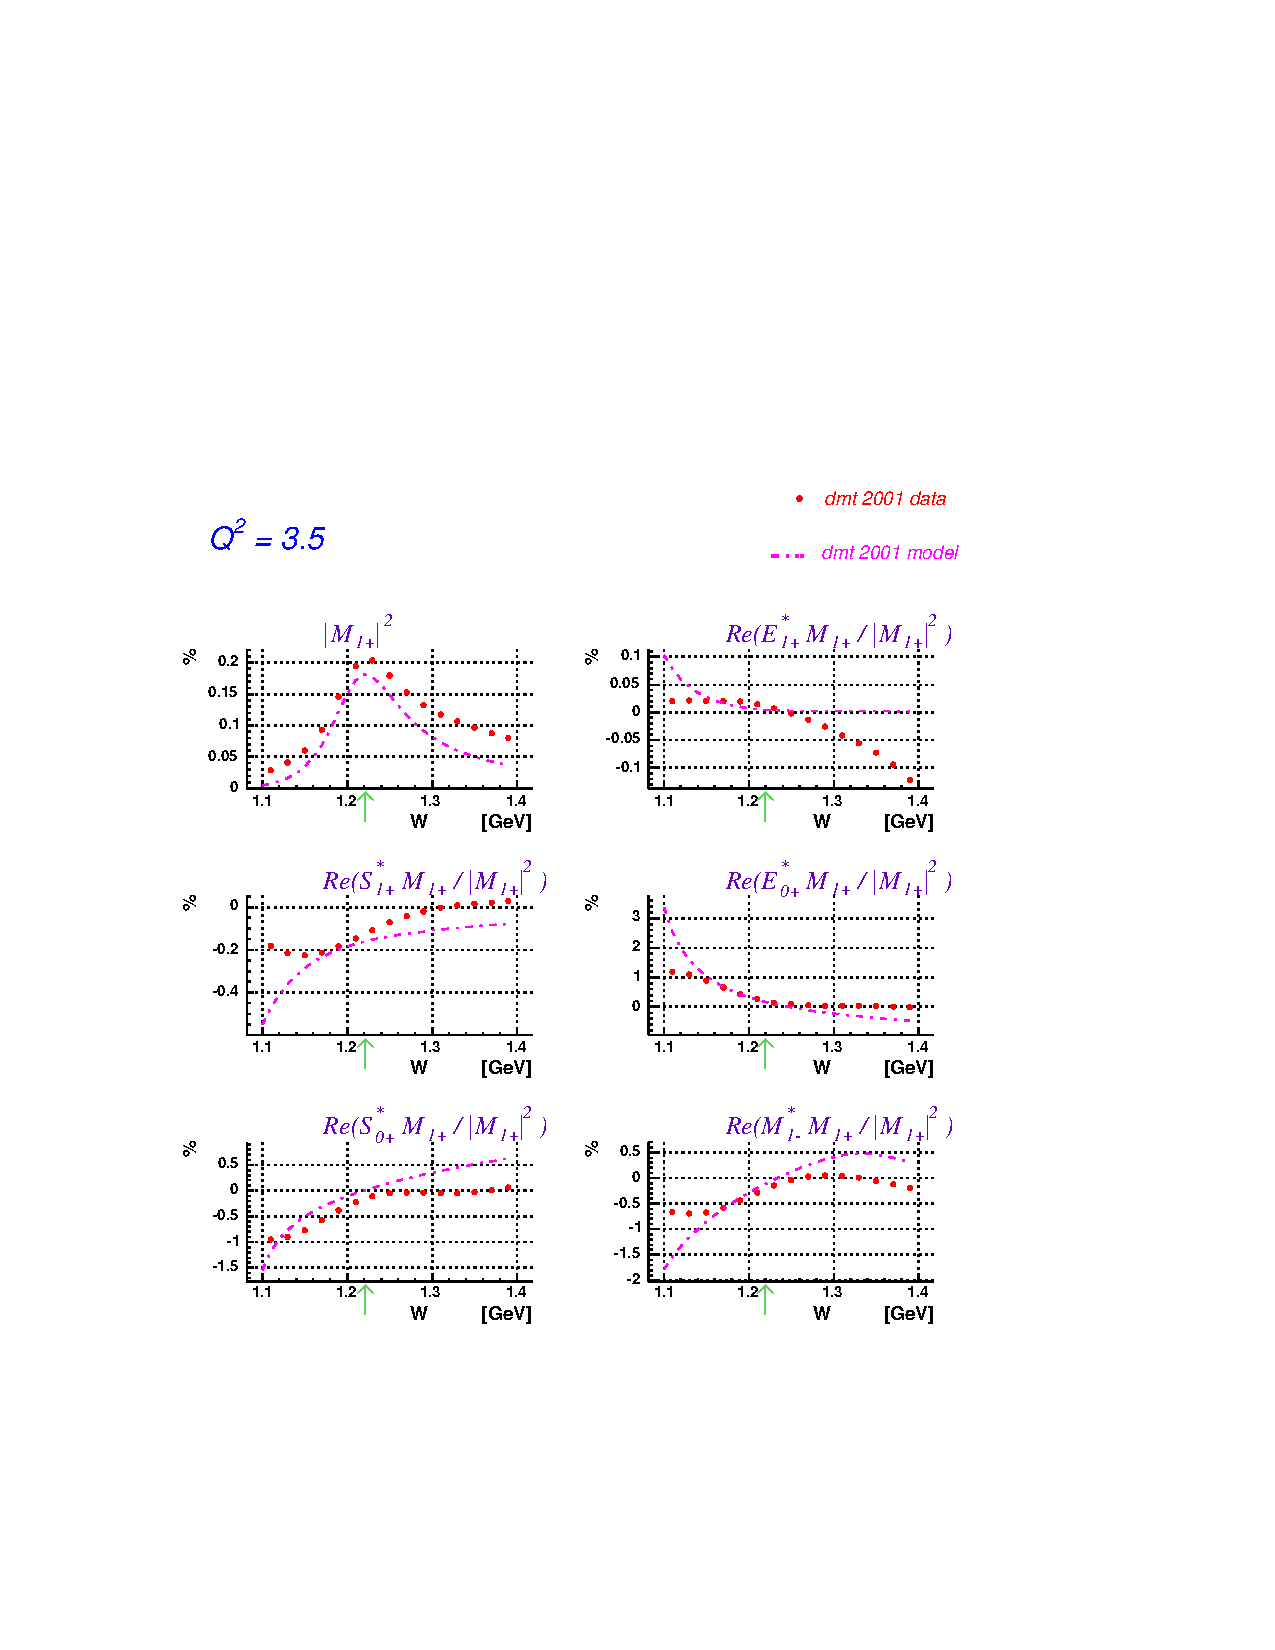
\includegraphics[width = 15cm, bb=60 100 540 600]{analysis/img/multipoles_q2_3.5_data2}
  \caption[Comparison between the model (dashed blue line) and extracted (red points) multipole ratios for DMT 2001]
          { Comparison between the model and extracted multipole ratios for DMT 2001 at $Q^2$ = $3.5$ GeV$^2$. }
 \label{fig:dmt_comp}
\end{center}
\end{figure}

\cia
The difference between the extracted multipole with the
model prediction at the $\Delta$ peak is illustrated in \F{fig:error_rm} for $E_{1+}/M_{1+}$ and in \F{fig:error_rs} for $S_{1+}/M_{1+}$.
\begin{figure}[h]
 \begin{center}
 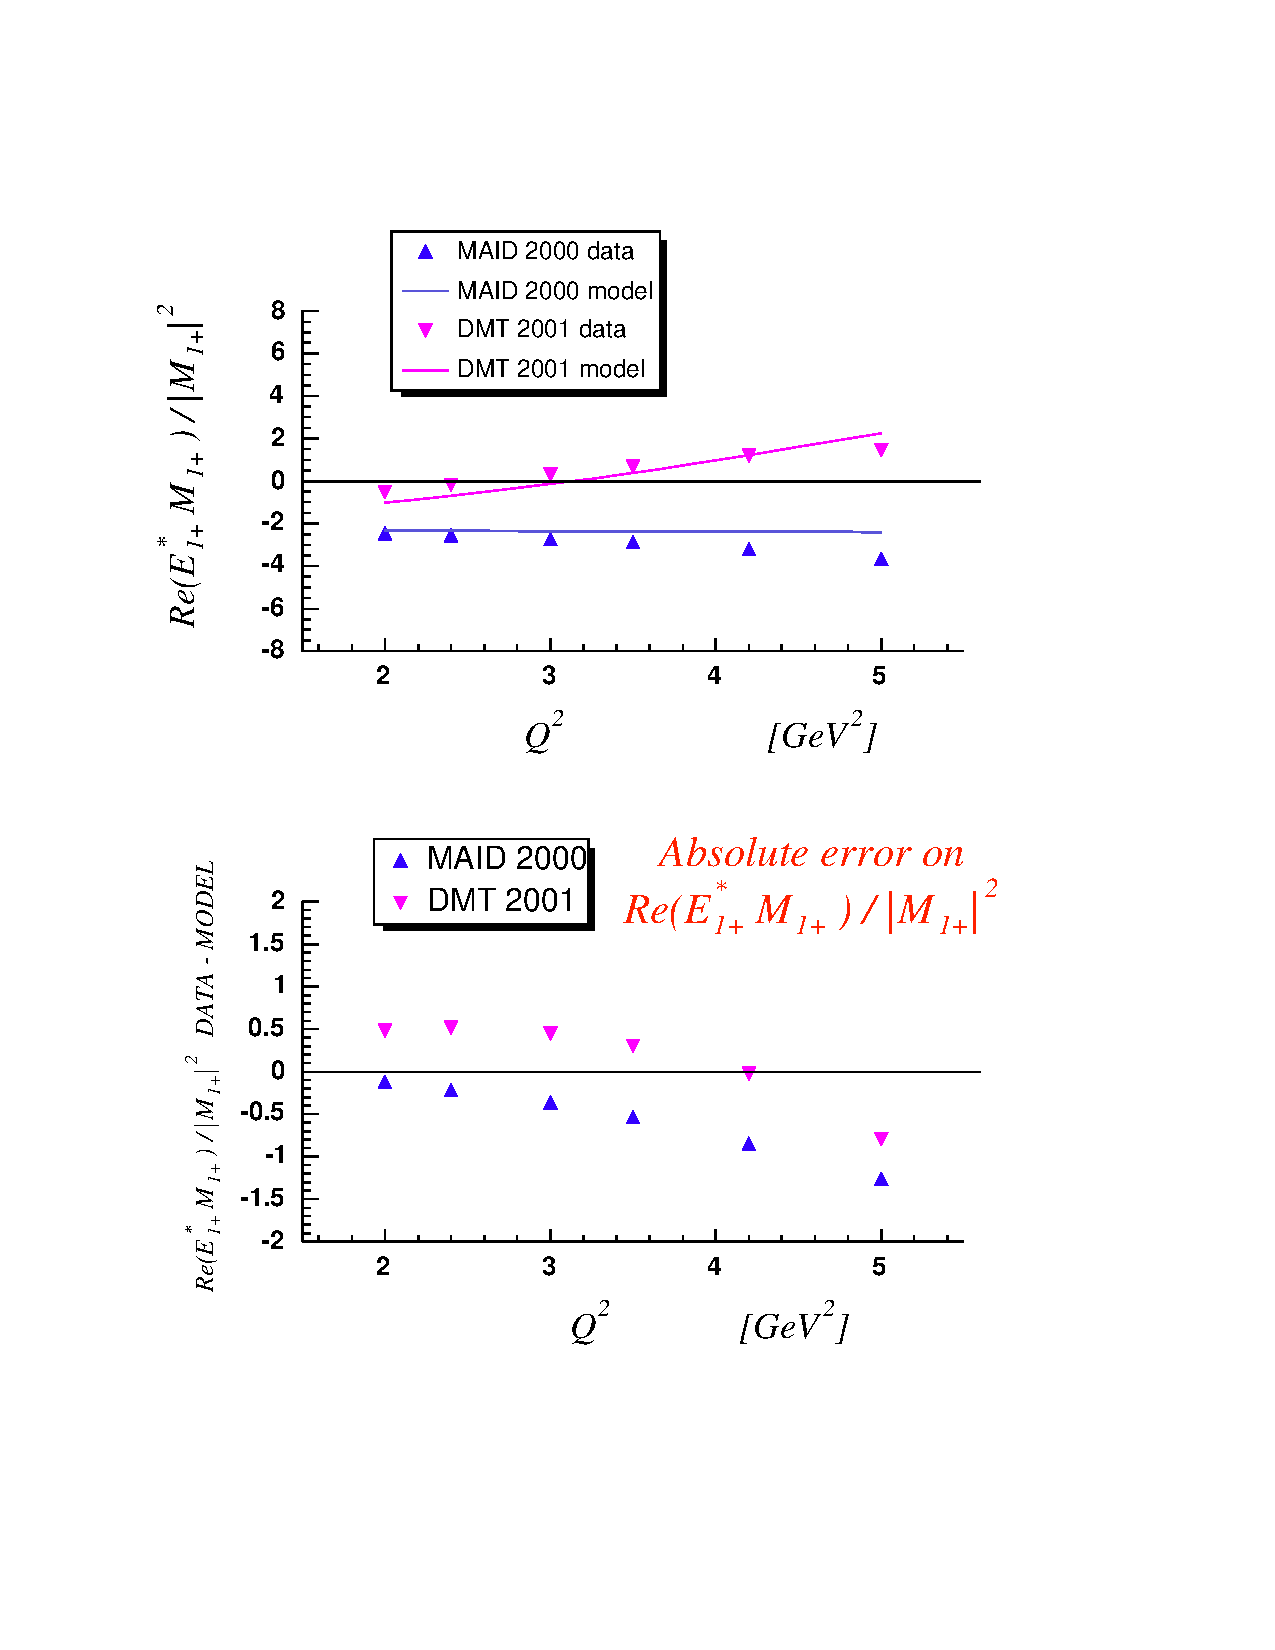
\includegraphics[width = 12cm, bb=30 130 560 720]{analysis/img/error_rm} 
  \caption[Model and extracted $E_{1+}/M_{1+}$ as a function of $Q^2$]
          {  Model and $M_{1+}$ dominance extracted $E_{1+}/M_{1+}$ as a function of $Q^2$. Top: 
	              the points are the value from the fit and the approximations described in
		      the text. The lines
		      are the model prediction. Bottom: absolute difference between between
		      extracted value and model prediction.}
 \label{fig:error_rm}
\end{center}
\end{figure}

When MAID is used the ratio $E_{1+}/M_{1+}$ is always underestimated, starting
at $\sim 0.2\%$ at $Q^2=2$ GeV$^2$ and up to $\sim 1.2\%$ at $Q^2=5$ GeV$^2$.
When DMT is used a rather constant overestimation by $\sim 0.5\%$ of $E_{1+}/M_{1+}$ up to $Q^2=3.5$ GeV$^2$ is obtained.
At $Q^2=4.2$ the value extracted is the same as in the model but at $Q^2=5$ $E_{1+}/M_{1+}$ is underestimated
by $\sim 0.8\%$.

As regarding $S_{1+}/M_{1+}$, the extraction from both models yelds a rather significant overestimation 
increasing in value with $Q^2$.
 
\begin{figure}[h]
 \begin{center}
 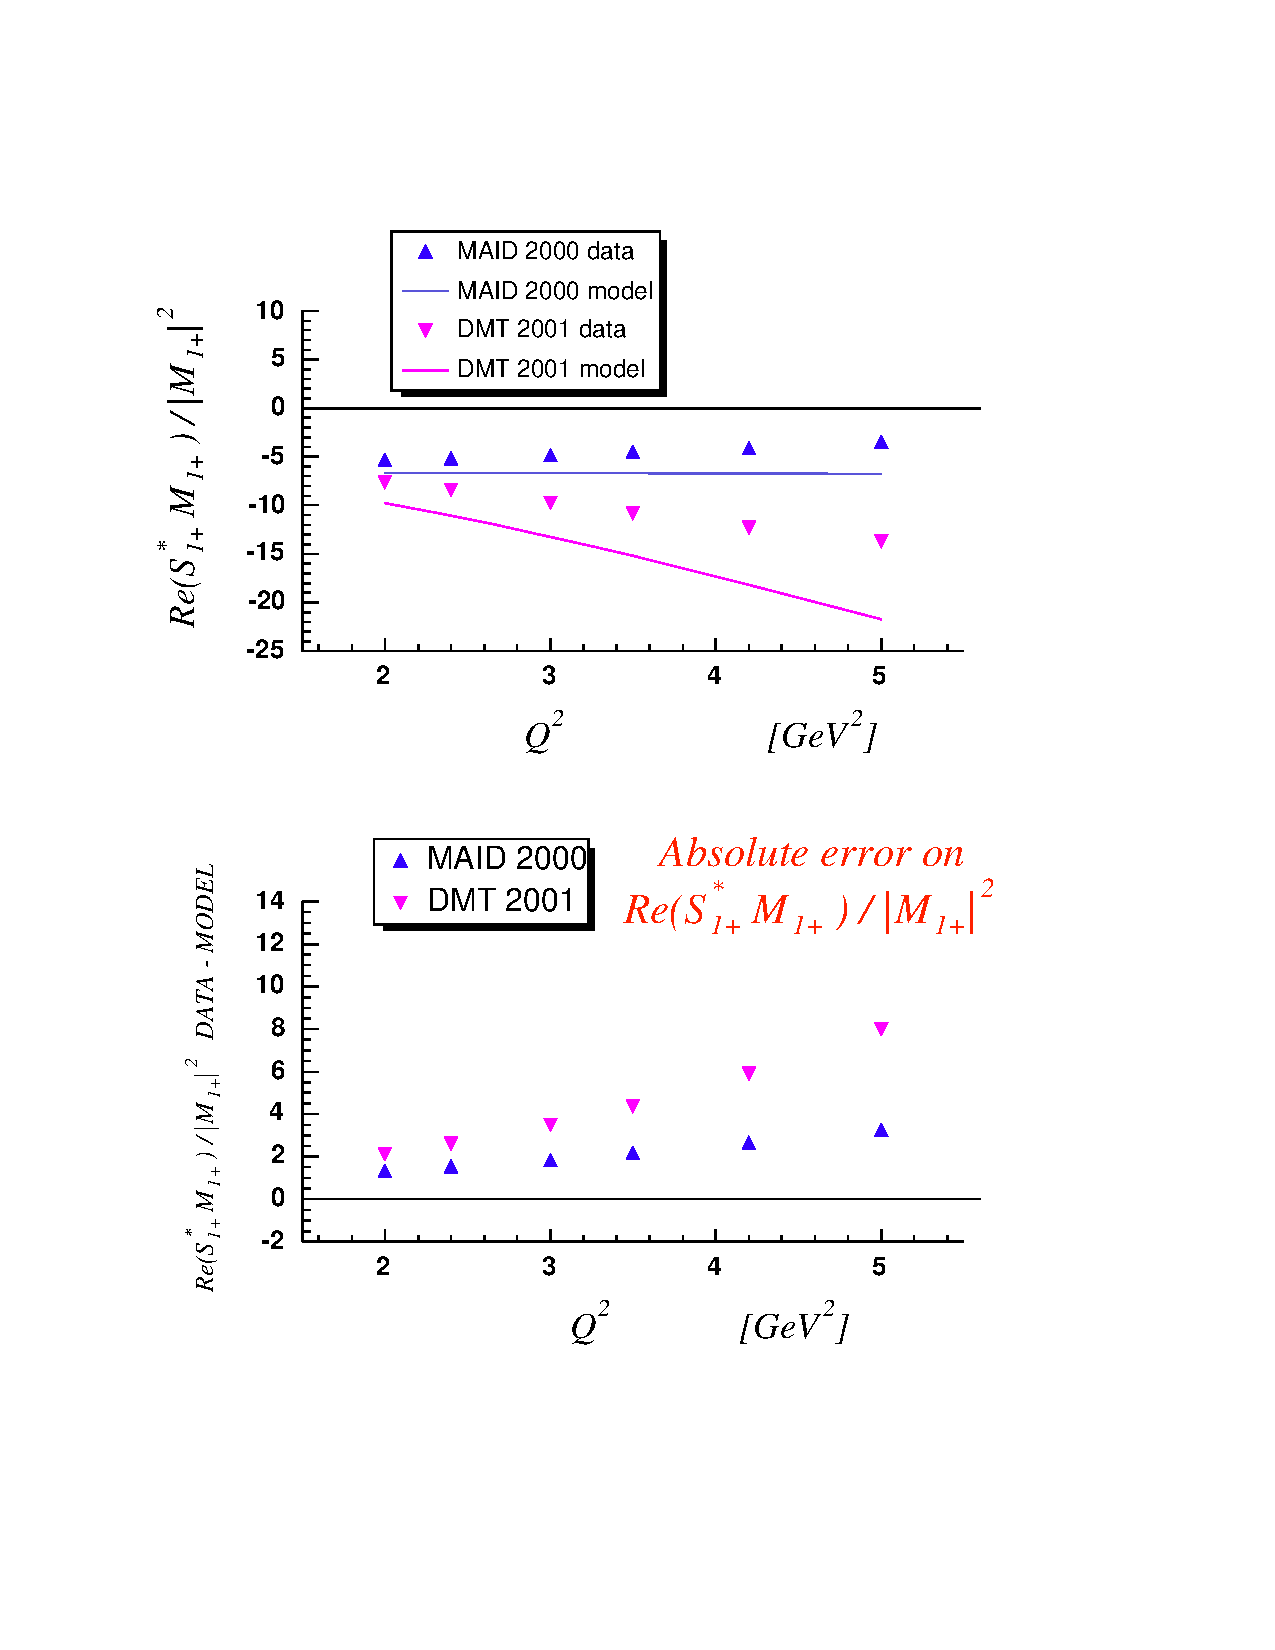
\includegraphics[width = 12cm, bb=30 130 560 720]{analysis/img/error_rs} 
  \caption[Model and extracted $S_{1+}/M_{1+}$ as a function of $Q^2$]
          {  Model and $M_{1+}$ dominance extracted $S_{1+}/M_{1+}$ as a function of $Q^2$. Top: 
	              the points are the value from the fit and the approximations described in
		      the text. The lines
		      are the model prediction. Bottom: absolute difference between between
		      extracted value and model prediction.}
 \label{fig:error_rs}
\end{center}
\end{figure}


















